
\documentclass[aspectratio=169]{beamer}

\mode<presentation> {
\usetheme{Madrid}
}

\usepackage{graphicx}
\usepackage{booktabs}
\usepackage[czech]{babel}
\usepackage[utf8]{inputenc}
\usepackage{hyperref}

\title[Intuicionismus]{Úvod do Intuicionistické logiky a konstruktivismu}

\author{Bc. Viet Bach Nguyen}
\institute[KIZI] {
    Vysoká škola ekonomická v Praze \\
    \medskip
    \textit{nguv03@vse.cz}
}
\date{14. prosince 2016}

\begin{document}

\begin{frame}
\titlepage
\end{frame}

\begin{frame}
\frametitle{Obsah}
\tableofcontents
\end{frame}

\section{Historie} 

\begin{frame}
\frametitle{Historie}
\begin{columns}
\column{0.75\textwidth}

\begin{itemize}
\item 2. pol. 19. stol. -- matematická krize
    
    \begin{itemize}
    \item Pokusy o re-stabilizaci: 
        \begin{itemize}
        \item Gottlob Frege (1848--1925) (DE), 
        \item Bertrand Russel (1872--1970) (GB)
        \end{itemize}
    \end{itemize}

    \begin{itemize}
    \item Nestabilní základy připouštějí různé matematické paradoxy 

        \begin{itemize}
        \item Holič ze Sevilly
        \item Uvažujme množinu množin, které nejsou prvkem sama sebe. Je tato množina svým prvkem?
        \end{itemize}
    
    \end{itemize}

\item Co je tím správným základem pro matematiku? Logika?
    \begin{itemize}
    \item Co je to axiom?
    \item Jednoduchá tvrzení, která se \uv{nemusí dokázat}
    \item Nelze dokázat úplně všechno dokola
    \end{itemize}

\end{itemize}

\column{0.25\textwidth}

\begin{figure}
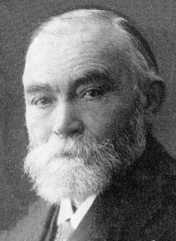
\includegraphics[scale=0.45]{frege}
\end{figure}

\begin{figure}
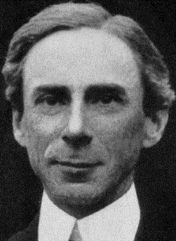
\includegraphics[scale=0.45]{russel}
\end{figure}
    
\end{columns}
\end{frame}





\begin{frame}
\frametitle{Historie}
\begin{columns}
\column{0.75\textwidth}
\begin{itemize}
\item David Hilbert (1862--1943) (DE):
\item Axiomatické systémy, které k absurditám nevedly
\item Nestabilní základy připouštějí různé matematické paradoxy 
\item Soubor axiomů, na jejichž základě nelze dokázat pravdivost $A \land \neg A$, je bezespornou teorií
\end{itemize}

\column{0.25\textwidth}
\begin{figure}
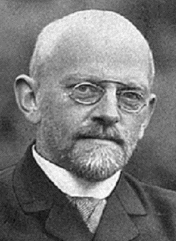
\includegraphics[scale=0.45]{hilbert}
\end{figure}
\uv{Není pravda, že existuje jen jedna správná matematika}
\end{columns}
\end{frame}




\begin{frame}
\frametitle{Historie}
\begin{columns}
\column{0.75\textwidth}
\begin{itemize}
\item Luitzen Brouwer (1881--1966) (NL)
\item Axiomatické budování matematiky je zcela \textbf{mylné}
\item Zakladatel matematického intuicionicismu
\item Základem matematiky má být \textit{intuice}
    \begin{itemize}
    \item přirozená čísla, matematická indukce
    \item operace jako sčítání, násobení apod. se nazývají \textit{konstrukce}
    \item matematika je vědou o konstrukcích v matematikově mysli
    \item neoprávněné matematické postupy vycházejí z matematického \textbf{platonismu}
    \item např. důkaz sporem je neintuitivní a neoprávněný, protože nedává návod, jak najít objekt, který má existovat
    \end{itemize}
\item Ve skutečnosti odmítal budovat matematiku pomocí jakékoli logiky, protože logika zachycuje pouze vlastnosti našeho jazyka
\end{itemize}

\column{0.25\textwidth}
\begin{figure}
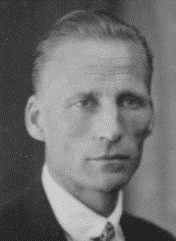
\includegraphics[scale=0.45]{brouwer}
\end{figure}
\end{columns}
\end{frame}


\section{Intuinicionistická logika}

\begin{frame}
\frametitle{Intuicionistická logika}
\begin{columns}
\column{0.6\textwidth}
\begin{itemize}
\item Chceme-li dokázat existenci objektu, musíme jej zkonstruovat
\item Může se stát, že neumíme zkonstruovat objekt ani dokázat jeho neexistenci
\item Zde \textbf{neplatí} zákon vyloučeného třetího!
    \begin{itemize}
    \item $A \lor B$ je dokázána pouze v případě, že je dokázán alespoň jeden z výroků $A, B$
    \item $A \lor \neg A$ nemusí být vždy pravdivé jako v klasické logice, tj. když není pravdivý ani $A$, ani $\neg A$
    \end{itemize}
\end{itemize}

\column{0.4\textwidth}
\begin{figure}
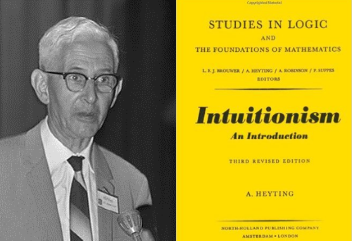
\includegraphics[scale=0.45]{heyting}
\end{figure}
\small
\begin{itemize}
\item Arend Heyting (1898--1980) (NL)
\item \uv{nikdy nebude možno matematicky přesně dokázat, že daná soustava axiómů skutečně obsahuje všechny platné metody důkazu}
\end{itemize}
\end{columns}
\end{frame}




\begin{frame}
\frametitle{Kolmogorova logika problému}
\begin{columns}
\column{0.8\textwidth}
\begin{itemize}
\item Andrey Kolmogorov (1903--1987) (RU)
\item Neuvažovat o výrocích, nýbrž problémech

\begin{table}
\begin{tabular}{ r l }
$\neg A$ & problém $A$ je neřešitelný \\ 
$A \land B$ & oba problémy, $A$ i $B$, jsou řešitelné \\
$A \lor B$ & $A$ je řešitelný nebo B je řešitelný \\
$A \Rightarrow B$ & je-li vyřešen problém $A$, je vyřešen i problém $B$ \\
$A \Leftrightarrow B$ & zkratka za $(A \Rightarrow B) \land (B \Rightarrow A)$ \\
\end{tabular}
\end{table}

\item \uv{řešitelný} zn. \uv{umíme zkonstruovat řešení}
\item \uv{neřešitelný} zn. \uv{umíme dokázat, že žádné řešení neexistuje}
\item \uv{nevím} zn. \uv{problém vyřešit neumíme, ani nevíme, jestli má řešení}
\item neplatí zákon vyloučeného třetího!
\end{itemize}

\column{0.20\textwidth}
\begin{figure}
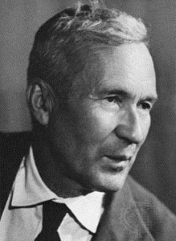
\includegraphics[scale=0.45]{kolmogorov}
\end{figure}
\end{columns}
\end{frame}




\begin{frame}
\frametitle{Inuticionistická logika -- příklad}
\begin{itemize}
\item Uvažujme jednoduchou formuli $A \Leftrightarrow \neg \neg A$
\item Tj. $(A \Rightarrow \neg \neg A) \land (\neg \neg A \Rightarrow A)$
\item První implikace
    \begin{itemize}
    \item je-li $A$ pravdivé, známe způsob, jak nalézt řešení problému $A$
    \item ovšem tím je dokázáno, že není neřešitelný
    \item tzn., že je dokázáno, že problém $\neg A$ je neřešitelný
    \item takže celá první implikace platí
    \end{itemize}
\item Druhá implikace
    \begin{itemize}
    \item $\neg \neg A$ říká, že umíme dokázat, že nelze dokázat neřešitelnost problému $A$
    \item ale z toho však ještě nijak neplyne, že problém $A$ už umíme vyřešit!
    \end{itemize}
\item Takže \textbf{celá formule} v Kolmogorově interpretaci \textbf{neplatí}
\end{itemize}
\end{frame}




\begin{frame}
\frametitle{Inuticionistická logika -- shrnutí}
\begin{itemize}
\item vychází pouze z toho, co opravdu víme (intuice), drží se přísně jen aktuálního vědění
\item zatímco u klasické logiky i když zrovna nevím, zda tvrzení je či není pravdivé, ono pravdivé nebo nepravdivé je

\begin{table}
\begin{tabular}{ r l }
$A$ & existuje konstrukce důkazu pro $A$ ($A$ je dokazatelná důkazem) \\ 
$\neg A$ & oba problémy, $A$ i $B$, jsou řešitelné \\
$A \lor \neg A$ & nemusí být vždy pravdivé, tj. musí být alespoň jeden člen disjunkce pravdivý \\
$\neg \neg A$ & není dokázána negace $A$, to ale neznamená, že je dokázána $A$ \\
\end{tabular}
\end{table}
\end{itemize}
\end{frame}




\begin{frame}
\frametitle{Inuticionistická logika -- shrnutí}
\begin{itemize}
\item IL připouští, že jsou tvrzení, která nemají ani jednu pravdivostní hodnotu, a jelikož tuto hodnotu neznáme, není zkonstruován ani jejich důkaz ani jejich vyvrácení
\item má snadno zdůvodnitelné principy
\item jenže není možné v ní dokázat mnoho věcí, které v klasické logice dokázat lze

\end{itemize}
\end{frame}




\begin{frame}
\frametitle{Reference}
\footnotesize{
\begin{thebibliography}{99}
\bibitem{link1} \url{http://atrey.karlin.mff.cuni.cz/~ansa/neklasiky/intuic.pdf}
\bibitem{link2} \url{https://mks.mff.cuni.cz/archive/26/9.pdf}
\bibitem{link3} \url{https://www.esf.kfi.zcu.cz/logika/opory/lof/prezentace/13.pdf}
\bibitem{link4} \url{https://plato.stanford.edu/entries/logic-intuitionistic/}
\bibitem{link5} \url{https://www.illc.uva.nl/Research/Publications/Reports/PP-2006-25.text.pdf} 
\bibitem{link6} \url{http://aleteya.cs.buap.mx/~jlavalle/papers/van\%20Dalen/Intuitionistic\%20Logic.pdf}
\end{thebibliography}
}
\end{frame}





\begin{frame}
\Huge{\centerline{Děkuji za pozornost}}
\end{frame}


\end{document}